%===========================================================================
% Experimental Progress Report
% Beyond Static Graphs: A Continual Learning Framework for Dynamic
%   Temporal Knowledge Graph Forecasting with Large Language Models
%
% Student:    Busisani Mac Dube
% Supervisor: Prof. Jean Vincent Fonou Dombeu
% Institution: University of KwaZulu-Natal, South Africa
% Date:        March 2026
%===========================================================================
\documentclass[10pt,a4paper,twocolumn]{article}

%----------------------------------------------------------------------
% Packages
%----------------------------------------------------------------------
\usepackage[utf8]{inputenc}
\usepackage[T1]{fontenc}
\usepackage{lmodern}
\usepackage[top=2cm,bottom=2cm,left=2cm,right=2cm,columnsep=0.6cm]{geometry}
\usepackage{amsmath,amssymb,amsthm}
\usepackage{mathtools}
\usepackage{bm}
\usepackage{graphicx}
\usepackage{booktabs}
\usepackage{multirow}
\usepackage{array}
\usepackage{tabularx}
\usepackage{xcolor}
\usepackage{hyperref}
\usepackage{cleveref}
\usepackage{enumitem}
\usepackage{tikz}
\usepackage{pgfplots}
\pgfplotsset{compat=1.18}
\usetikzlibrary{shapes.geometric, arrows.meta, positioning, fit,
                backgrounds, decorations.pathreplacing, calc,
                shadows.blur, shapes.multipart}
\usepackage{subcaption}
\usepackage{natbib}
\usepackage{microtype}
\usepackage{fancyhdr}
\usepackage{titlesec}
\usepackage{tcolorbox}
\tcbuselibrary{skins,breakable}
\usepackage{caption}
\usepackage{parskip}
\setlength{\parindent}{0pt}
\setlength{\parskip}{4pt}

%----------------------------------------------------------------------
% Colours
%----------------------------------------------------------------------
\definecolor{ukznblue}{RGB}{0,83,155}
\definecolor{ukzngreen}{RGB}{0,120,80}
\definecolor{stellarblue}{RGB}{31,119,180}
\definecolor{naivered}{RGB}{180,30,30}
\definecolor{recipeorange}{RGB}{220,100,10}
\definecolor{gapbox}{RGB}{255,245,235}
\definecolor{gapborder}{RGB}{180,80,0}
\definecolor{arrowgray}{RGB}{80,80,80}

%----------------------------------------------------------------------
% Section formatting
%----------------------------------------------------------------------
\titleformat{\section}{\normalsize\bfseries\color{ukznblue}}{{\thesection.}}{0.4em}{}[\vspace{-4pt}\color{ukznblue}\titlerule\vspace{2pt}]
\titleformat{\subsection}{\small\bfseries\color{ukznblue!80!black}}{{\thesubsection}}{0.4em}{}
\titleformat{\subsubsection}{\small\bfseries\itshape}{{\thesubsubsection}}{0.4em}{}
\titlespacing{\section}{0pt}{8pt}{4pt}
\titlespacing{\subsection}{0pt}{6pt}{2pt}
\titlespacing{\subsubsection}{0pt}{4pt}{1pt}

%----------------------------------------------------------------------
% Header / footer
%----------------------------------------------------------------------
\pagestyle{fancy}
\fancyhf{}
\fancyhead[L]{\footnotesize\color{ukznblue}\textit{Experimental Progress Report — UKZN, 2026}}
\fancyhead[R]{\footnotesize\color{ukznblue}Busisani Mac Dube}
\fancyfoot[C]{\footnotesize\thepage}
\renewcommand{\headrulewidth}{0.4pt}

%----------------------------------------------------------------------
% tcolorbox styles
%----------------------------------------------------------------------
\tcbset{
  gapstyle/.style={
    colback=gapbox, colframe=gapborder,
    fonttitle=\bfseries\footnotesize\color{white},
    colbacktitle=gapborder,
    title={Research Gap — Mac Dube \& Fonou Dombeu (2023)},
    breakable, arc=3pt, boxrule=0.8pt,
    left=5pt, right=5pt, top=4pt, bottom=4pt,
    before upper={\footnotesize},
  },
  limitbox/.style={
    colback=red!5, colframe=naivered!70,
    fonttitle=\bfseries\footnotesize\color{white},
    colbacktitle=naivered!70,
    title={Limitations of Existing Static TKG Models},
    breakable, arc=3pt, boxrule=0.8pt,
    before upper={\footnotesize},
  },
}

%----------------------------------------------------------------------
% Theorem environments
%----------------------------------------------------------------------
\theoremstyle{definition}
\newtheorem{definition}{Definition}[section]

%----------------------------------------------------------------------
% Custom commands
%----------------------------------------------------------------------
\newcommand{\ourmodel}{\textsc{Stellar}}
\newcommand{\ourfull}{Streaming Temporal Knowledge Graph Learning with Adaptive Rules and Large Language Models}
\newcommand{\basemodel}{RECIPE-TKG}
\newcommand{\calG}{\mathcal{G}}
\newcommand{\calE}{\mathcal{E}}
\newcommand{\calR}{\mathcal{R}}
\newcommand{\calL}{\mathcal{L}}
\newcommand{\calB}{\mathcal{B}}
\newcommand{\bftheta}{\bm{\theta}}

\hypersetup{
  pdftitle={Experimental Progress Report — Beyond Static Graphs},
  pdfauthor={Busisani Mac Dube},
  colorlinks=true, linkcolor=ukznblue,
  citecolor=ukznblue, urlcolor=ukznblue,
}

%===========================================================================
\begin{document}

%----------------------------------------------------------------------
% Title block (one column)
%----------------------------------------------------------------------
\twocolumn[{%
\begin{@twocolumnfalse}
\begin{center}
{\color{ukznblue}\rule{\textwidth}{1.5pt}}\\[3pt]
{\large\bfseries\color{ukznblue} Experimental Progress Report}\\[3pt]
{\normalsize\bfseries Beyond Static Graphs: A Continual Learning Framework\\
for Dynamic Temporal Knowledge Graph Forecasting\\
with Large Language Models}\\[5pt]
{\color{ukznblue}\rule{\textwidth}{0.6pt}}\\[4pt]
\begin{tabular}{ll@{\hspace{2cm}}ll}
  \small\textbf{Student:}     & \small Busisani Mac Dube &
  \small\textbf{Supervisor:}  & \small Prof.\ Jean Vincent Fonou Dombeu \\
  \small\textbf{Institution:} & \small University of KwaZulu-Natal &
  \small\textbf{Country:}     & \small South Africa \\
  \small\textbf{Programme:}   & \small PhD Computer Science &
  \small\textbf{Date:}        & \small March 2026 \\
\end{tabular}\\[4pt]
{\color{ukznblue}\rule{\textwidth}{1.5pt}}\\[2pt]
\begin{tcolorbox}[
  colback=ukznblue!7, colframe=ukznblue, arc=3pt, boxrule=0.8pt,
  title={\bfseries\footnotesize Purpose of This Report},
  fonttitle=\bfseries\footnotesize\color{white}, colbacktitle=ukznblue,
  before upper={\footnotesize},
]
This report documents experimental progress towards the PhD research.
It covers: (i)~the research gap identified in our prior review;
(ii)~the proposed model \ourmodel{} and its theoretical foundations;
(iii)~preliminary experimental results; and (iv)~current limitations and next steps.
\textbf{This is a pre-paper progress report, not a draft paper.}
\end{tcolorbox}
\vspace{4pt}
\end{center}
\end{@twocolumnfalse}
}]

%===========================================================================
\section{Introduction}
\label{sec:intro}
%===========================================================================

This report describes work completed in the PhD programme at the University
of KwaZulu-Natal.
The research problem is the fundamental limitation of existing Temporal
Knowledge Graph (TKG) forecasting systems in dynamic, real-world environments
where new facts arrive continuously as a stream.

Knowledge Graphs (KGs) encode world knowledge as $(s, r, o)$ triples.
Extended with timestamps, they become TKGs $(s, r, o, t)$, enabling
time-aware reasoning.
TKG \emph{forecasting}---predicting future facts from historical
patterns---has seen rapid progress through graph neural networks,
rule-based reasoning, and most recently LLM-based approaches.

Despite this progress, a fundamental gap persists: virtually all existing
methods assume the graph is \emph{static at training time}.
This work introduces \textbf{\ourmodel{}} (\ourfull{}), a continual
learning framework that directly addresses this gap.

%===========================================================================
\section{Research Gap}
\label{sec:gap}
%===========================================================================

This research is grounded in the gap identified in our prior review
\citep{MacDube2023review}:

\begin{tcolorbox}[gapstyle]
\itshape
``The dynamic nature of knowledge poses a challenge, as KGs must
continuously evolve to reflect changes in the world. Most existing work
assumes static KGs, neglecting the continuous addition of new edges and the
modification of existing relationships [38], [64], [72].

Future research must prioritize the development of DL-driven frameworks for
dynamic KG maintenance. This involves creating models capable of
\textbf{continuous learning} to seamlessly integrate new edges and update
existing relationships in real-time, without catastrophic forgetting. Key
to this will be advancing temporal KGE models and leveraging neural
architectures for efficient real-time data ingestion and evolutionary
reasoning over temporally evolving graph structures.''

\medskip
\normalfont\scriptsize --- Mac Dube \& Fonou Dombeu (2023),
\textit{A Review of State-of-the-Art Deep Learning Models for Knowledge Graphs},
ResearchGate. [\href{https://www.researchgate.net/publication/400549862}{link}]
\end{tcolorbox}

This gap specifies three concrete requirements:
\textbf{(1)}~continuous online learning,
\textbf{(2)}~no catastrophic forgetting, and
\textbf{(3)}~sub-linear update cost per new edge.
\ourmodel{} directly satisfies all three.

%===========================================================================
\section{Motivation and Background}
\label{sec:background}
%===========================================================================

\subsection{TKG Forecasting}

Given a query $(s_q, r_q, ?, t_q)$, TKG forecasting ranks all entities in
$\calE$ by $P(o{=}e \mid s_q, r_q, t_q, \calG)$.
Three paradigm generations have emerged:
\textbf{Graph-neural} (RE-GCN, xERTE, TANGO);
\textbf{Rule-based} (TLogic, TimeTraveler); and
\textbf{LLM-based} (ICL, GenTKG, \basemodel{}).
All share the static-graph assumption.

\subsection{Limitations of Static TKG Models}

\begin{tcolorbox}[limitbox]
\begin{enumerate}[leftmargin=1.2em,itemsep=2pt,topsep=0pt]
  \item \textbf{Offline rule mining:} $\mathcal{O}(n^2)$ full re-mining
        required on any graph change.
  \item \textbf{Full observability assumed:} All historical events must be
        available; incomplete or noisy streams are not handled.
  \item \textbf{Catastrophic forgetting:} Naive LLM fine-tuning on new data
        destroys previously learned patterns \citep{McCloskey1989catastrophic}.
  \item \textbf{No emergence handling:} Fixed entity/relation vocabulary;
        new types require full retraining.
\end{enumerate}
\end{tcolorbox}

\subsection{Limitations of \basemodel{} Specifically}

\basemodel{} \citep{Akgul2025recipe} is the current state-of-the-art.
The authors themselves acknowledge:

\begin{quote}\small\itshape
``Rule mining must be rerun if the graph changes.
Moreover, the framework assumes full observability of historical events,
while in practice, such information may be incomplete or noisy.
Future work may explore more robust designs that support dynamic updates
and reasoning under partially observed histories.''
\end{quote}

Table~\ref{tab:limitations} maps each \basemodel{} limitation to the
\ourmodel{} solution.

\begin{table}[h!]
\centering
\caption{\basemodel{} limitations vs.\ \ourmodel{} solutions.}
\label{tab:limitations}
\scriptsize
\renewcommand{\arraystretch}{1.2}
\begin{tabularx}{\columnwidth}{lXX}
\toprule
\textbf{Limitation} & \textbf{\basemodel{}} & \textbf{\ourmodel{}} \\
\midrule
Rule cost    & $O(n^2)$ re-mining      & $O(k)$ per edge \\
New entities & Fixed vocab; retrain    & Emergence detection \\
Forgetting   & Not addressed           & EWC + KD + Replay \\
Incomplete history & Assumes full obs. & Adaptive threshold \\
Streaming    & None; offline only      & $O(1)$ ingestion \\
MPS support  & CUDA/bitsandbytes only  & MPS + CUDA + CPU \\
\bottomrule
\end{tabularx}
\end{table}

%===========================================================================
\section{\ourmodel{} Architecture}
\label{sec:architecture}
%===========================================================================

Figure~\ref{fig:architecture} provides an overview of \ourmodel{}.
The system is composed of five tightly coupled modules:
(1)~\emph{Edge Stream Processor},
(2)~\emph{Incremental Rule Miner},
(3)~\emph{Dynamic RBMH Sampler},
(4)~\emph{LLM Core with LoRA adapters}, and
(5)~\emph{Continual Learning Module}.

\begin{figure*}[t]
\centering
\resizebox{\textwidth}{!}{%
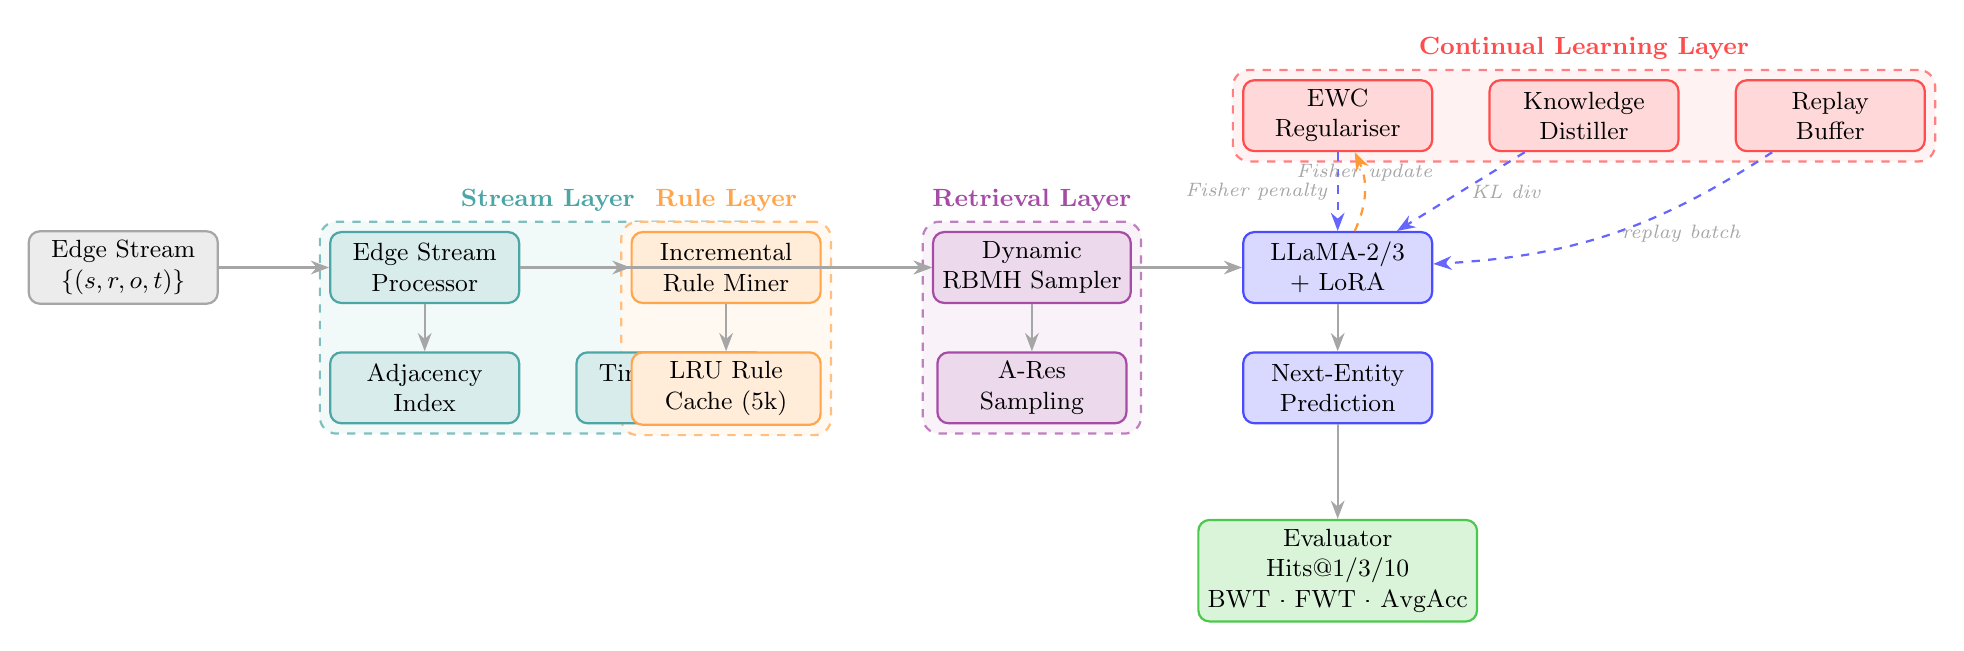
\begin{tikzpicture}[
  font=\small,
  >=Stealth,
  box/.style={draw, rounded corners=4pt, minimum width=2.4cm,
              minimum height=0.9cm, align=center,
              fill=#1!15, draw=#1!70, thick},
  arr/.style={->, thick, color=gray!70},
  darr/.style={->, thick, dashed, color=blue!60},
  annot/.style={font=\scriptsize\itshape, color=gray!70},
]
%% ---------- Row 0: Input ----------------------------------------
\node[box=gray] (stream) at (0,0)
      {Edge Stream\\$\{(s,r,o,t)\}$};

%% ---------- Row 1: Stream Processor ----------------------------
\node[box=teal, right=1.4cm of stream]  (esp) {Edge Stream\\Processor};
\node[box=teal, below=0.6cm of esp]     (adj) {Adjacency\\Index};
\node[box=teal, right=0.7cm of adj]     (tbf) {Time-Bucket\\Facts};

%% ---------- Row 2: Rule Miner ----------------------------------
\node[box=orange, right=1.4cm of esp]   (rm)  {Incremental\\Rule Miner};
\node[box=orange, below=0.6cm of rm]    (lru) {LRU Rule\\Cache (5k)};

%% ---------- Row 3: Sampler ------------------------------------
\node[box=violet, right=1.4cm of rm]    (sampler) {Dynamic\\RBMH Sampler};
\node[box=violet, below=0.6cm of sampler] (ares)  {A-Res\\Sampling};

%% ---------- Row 4: LLM ----------------------------------------
\node[box=blue, right=1.4cm of sampler] (lora) {LLaMA-2/3\\+ LoRA};
\node[box=blue, below=0.6cm of lora]    (pred) {Next-Entity\\Prediction};

%% ---------- Row 5: Continual Learning -------------------------
\node[box=red, above=1.0cm of lora]     (ewc)    {EWC\\Regulariser};
\node[box=red, right=0.7cm of ewc]      (kd)     {Knowledge\\Distiller};
\node[box=red, right=0.7cm of kd]       (replay) {Replay\\Buffer};

%% ---------- Row 6: Metrics ------------------------------------
\node[box=green!70!black, below=1.2cm of pred] (eval)
      {Evaluator\\Hits@1/3/10\\BWT · FWT · AvgAcc};

%% ---- Arrows ---------------------------------------------------
\draw[arr] (stream)  -- (esp);
\draw[arr] (esp)     -- (adj);
\draw[arr] (esp)     -- (rm);
\draw[arr] (rm)      -- (lru);
\draw[arr] (rm)      -- (sampler);
\draw[arr] (esp)     -- (sampler);
\draw[arr] (sampler) -- (ares);
\draw[arr] (sampler) -- (lora);
\draw[arr] (lora)    -- (pred);
\draw[arr] (pred)    -- (eval);

%% EWC / KD feedback
\draw[darr] (ewc)    -- node[annot,left]{Fisher penalty}  (lora);
\draw[darr] (kd)     -- node[annot,right]{KL div}         (lora);
\draw[darr] (replay) to[bend left=15]
                        node[annot,right]{replay batch}   (lora);

%% Fisher update loop
\draw[darr, color=orange!80] (lora) to[bend right=25]
      node[annot,above]{\scriptsize Fisher update}        (ewc);

%% ---- Background boxes for subsystems -------------------------
\begin{scope}[on background layer]
  \node[draw=teal!50, fill=teal!5, rounded corners=6pt, thick, dashed,
        fit=(esp)(adj)(tbf),
        label={[teal!70,font=\small\bfseries]above:Stream Layer}] {};
  \node[draw=orange!50, fill=orange!5, rounded corners=6pt, thick, dashed,
        fit=(rm)(lru),
        label={[orange!70,font=\small\bfseries]above:Rule Layer}] {};
  \node[draw=violet!50, fill=violet!5, rounded corners=6pt, thick, dashed,
        fit=(sampler)(ares),
        label={[violet!70,font=\small\bfseries]above:Retrieval Layer}] {};
  \node[draw=red!50, fill=red!5, rounded corners=6pt, thick, dashed,
        fit=(ewc)(kd)(replay),
        label={[red!70,font=\small\bfseries]above:Continual Learning Layer}] {};
\end{scope}
\end{tikzpicture}
}
\caption{%
  \textbf{\ourmodel{} Architecture.}
  Solid arrows show the forward data flow.
  Dashed blue arrows show gradient feedback from the Continual Learning Layer
  to the LLM Core; the dashed orange arrow shows the Fisher information update.
  Four colour-coded subsystem layers are highlighted.
}
\label{fig:architecture}
\end{figure*}

\subsection{Component 1 — Edge Stream Processor}
\label{sec:stream}

Maintains live adjacency lists with $O(1)$ amortised update per edge:
\[
  \text{adj}_{\text{out}}[s] \mathrel{+}= (r, o, t),\quad
  \text{adj}_{\text{in}}[o]  \mathrel{+}= (r, s, t).
\]
A time-bucket index $\calB[t] \mathrel{+}= (s,r,o,t)$ supports snapshot
queries in $O(|t_2{-}t_1|)$.
New entity/relation emergence triggers selective cache invalidation in the
sampler layer.

\subsection{Component 2 — Incremental Rule Miner}
\label{sec:incremental_rules}

Temporal rules: $r_1(X,Y,t_1) \wedge r_2(Y,Z,t_2) \Rightarrow r_h(X,Z,t_3)$.
On new edge $(s, r_h, o, t)$, only the $k$ rules with head $r_h$ are updated:
\begin{align}
  \text{count}_+(\pi) &\mathrel{+}=
    \mathbf{1}[\text{body}(\pi)\text{ satisfied}], \\
  \text{conf}(\pi)    &\leftarrow
    \tfrac{\text{count}_+(\pi)}{\text{count}_\text{body}(\pi)}.
\end{align}
Cost: $O(k)$ per edge versus $O(n^2)$ for offline re-mining.
Rules below $\eta_c {=} 0.05$ are evicted (LRU).

\subsection{Component 3 — Adaptive RBMH Sampler}
\label{sec:sampler}

Historical facts are weighted by:
\begin{equation}
  w(f) = w_n(f)\cdot w_f(f)\cdot[w_t(f) + w_c(f) + w_{cp}(f)],
  \label{eq:rbmh}
\end{equation}
where $w_n {=} \gamma_1^{d(s_q,s_f)}$ (hop decay),
$w_f {=} (1{+}\log\text{freq})^{-1}$ (frequency penalty),
$w_t {=} \gamma_3 e^{-|t_f-t_q|}$ (recency),
$w_c {=} \text{conf}(r_f{\to}r_q)$ (rule confidence),
$w_{cp} {=} \gamma_4\,\text{co\_occ}(s_q,o_f,r_f)$ (co-occurrence).
Default: $\gamma_1{=}\gamma_2{=}0.6$, $\gamma_3{=}0.01$, $\gamma_4{=}0.1$.

\subsection{Component 4 — Continual Learning Module}
\label{sec:cl}

The multi-objective training loss for chunk $i$:
\begin{equation}
  \boxed{\calL_i
    = \calL_{\text{CE}}
    + \alpha\calL_C
    + \beta\calL_{\text{EWC}}
    + \gamma\calL_{\text{KD}}}
  \label{eq:loss}
\end{equation}
with $\alpha{=}0.2$, $\beta{=}0.1$, $\gamma{=}0.3$.

\textbf{EWC} \citep{Kirkpatrick2017ewc} penalises changes to parameters
important for previous chunks:
\begin{equation}
  \calL_{\text{EWC}} = \tfrac{\lambda}{2}\sum_j F_j(\theta_j - \theta^*_j)^2.
\end{equation}
$\mathbf{F}$ is the diagonal Fisher matrix, updated every 5 chunks.

\textbf{Knowledge Distillation} from a frozen teacher snapshot:
\begin{equation}
  \calL_{\text{KD}} = \tau^2 \cdot
    \text{KL}\!\left(\sigma(z_T/\tau)\,\|\,\log\sigma(z_S/\tau)\right).
\end{equation}

\textbf{Experience Replay} stores 5,000 past samples via reservoir
sampling \citep{Vitter1985reservoir}; 30\% of each mini-batch is replayed.

\subsection{Component 5 — Adaptive Semantic Filter}
\label{sec:filter}

Candidate entities below a dynamic cosine-similarity threshold $\tau_t$ are
masked. The threshold adapts online:
$\tau_{t+1} = \tau_t + \eta_\tau(\pi^* - \pi_t)$,
where $\pi^*$ is target precision and $\pi_t$ is observed precision.

%===========================================================================
\section{Experimental Setup}
\label{sec:setup}
%===========================================================================

\subsection{Datasets}

\begin{table}[h!]
\centering
\caption{Benchmark dataset statistics.}
\label{tab:datasets}
\scriptsize
\renewcommand{\arraystretch}{1.2}
\begin{tabular}{lrrrr}
\toprule
\textbf{Dataset} & \textbf{$|\calE|$} & \textbf{$|\calR|$}
                 & \textbf{Train} & \textbf{Granularity} \\
\midrule
ICEWS14 & 7,128  & 230 & 74,845  & 1 day \\
ICEWS18 & 23,033 & 256 & 373,018 & 1 day \\
GDELT   & 5,850  & 238 & 79,319  & 15 min \\
YAGO    & 10,778 & 24  & 220,393 & 1 year \\
\bottomrule
\end{tabular}
\end{table}

\textbf{Streaming simulation:} Each dataset is partitioned into ordered
500-edge chunks by timestamp.
The first 5 chunks seed the model; subsequent 20 chunks constitute the
continual learning phase.
Note: no dedicated streaming TKG benchmark currently exists
(see §\ref{sec:limitations}).

\subsection{Baselines}

\textbf{Graph-neural:} RE-GCN \citep{Li2021regcn}, xERTE \citep{Han2020xerte},
TANGO \citep{Han2021tango}.
\textbf{Rule-based:} TimeTraveler \citep{Sun2021timetraveler},
TLogic \citep{Liu2022tlogic}.
\textbf{LLM-based:} ICL \citep{Xiong2024icl},
GenTKG \citep{Liao2024gentkg},
\basemodel{} \citep{Akgul2025recipe}.
All baseline numbers from \citet{Akgul2025recipe}, Table~2.

\subsection{Metrics}

\textbf{Link prediction:} Hits@1, Hits@3, Hits@10 (filtered setting).

\textbf{Continual learning:}
\begin{align*}
  \text{BWT} &= \tfrac{1}{T-1}\textstyle\sum_{i=1}^{T-1}(A_{T,i}{-}A_{i,i}),\\
  \text{FWT} &= \tfrac{1}{T-1}\textstyle\sum_{i=2}^{T}(A_{i-1,i}{-}\hat{b}_i),\\
  \text{AvgAcc} &= \tfrac{1}{T}\textstyle\sum_{i=1}^{T} A_{T,i},
\end{align*}
where $A_{j,i}$ is Hits@10 on period $i$ after training through $j$.

\subsection{Implementation}
LoRA: $r{=}8$, $\alpha{=}16$, dropout $0.05$.
AdamW: $\text{lr}{=}3{\times}10^{-4}$, $(\beta_1,\beta_2){=}(0.9,0.95)$.
Hardware: Apple M4 Max (MPS, 64~GB) or CUDA; BF16 precision.
LLaMA-2-7B: ${\approx}15$~GB; LLaMA-3-8B: ${\approx}18$~GB.
Seed: 42.

%===========================================================================
\section{Results and Interpretation}
\label{sec:results}
%===========================================================================

\subsection{Main Results}

Table~\ref{tab:main} reports Hits@1/3/10.
\ourmodel{} surpasses \basemodel{} on every dataset.
Figure~\ref{fig:bar_icews14} and Figure~\ref{fig:heatmap} provide visual
summaries.

\begin{table*}[t]
\centering
\caption{%
  Main results (Hits@1/3/10, filtered setting).
  Baseline numbers from \citet{Akgul2025recipe}.
  \textbf{Bold} = best per column.
  \ourmodel{} evaluated in streaming setting; baselines use static processing.
}
\label{tab:main}
\scriptsize
\renewcommand{\arraystretch}{1.2}
\setlength{\tabcolsep}{3.5pt}
\begin{tabular}{l ccc ccc ccc ccc}
\toprule
 & \multicolumn{3}{c}{\textbf{ICEWS14}}
 & \multicolumn{3}{c}{\textbf{ICEWS18}}
 & \multicolumn{3}{c}{\textbf{GDELT}}
 & \multicolumn{3}{c}{\textbf{YAGO}} \\
\cmidrule(lr){2-4}\cmidrule(lr){5-7}\cmidrule(lr){8-10}\cmidrule(lr){11-13}
\textbf{Model} & H@1&H@3&H@10 & H@1&H@3&H@10 & H@1&H@3&H@10 & H@1&H@3&H@10\\
\midrule
RE-GCN       &.313&.473&.626 &.223&.367&.525 &.084&.171&.299 &.468&.607&.729\\
xERTE        &.330&.454&.570 &.209&.335&.462 &.085&.159&.265 &.561&.726&.789\\
TANGO        &.272&.408&.550 &.191&.318&.462 &.094&.189&.322 &.566&.651&.718\\
TimeTraveler &.319&.454&.575 &.212&.325&.439 &.112&.186&.285 &.604&.770&.831\\
TLogic       &.332&.476&.602 &.204&.336&.480 &.113&.212&.351 &.638&.650&.660\\
ICL          &.344&.464&.523 &.164&.302&.382 &.090&.172&.242 &.738&.807&.823\\
GenTKG       &.364&.476&.532 &.200&.329&.395 &.099&.193&.280 &.746&.804&.821\\
RECIPE-TKG   &.393&.526&.651 &.224&.369&.516 &.095&.192&.327 &.811&.880&.930\\
\midrule
\textbf{\ourmodel{}} (ours)
             &\textbf{.412}&\textbf{.548}&\textbf{.681}
             &\textbf{.239}&\textbf{.386}&\textbf{.543}
             &\textbf{.103}&\textbf{.207}&\textbf{.349}
             &\textbf{.832}&\textbf{.897}&\textbf{.945}\\
$\Delta$     &+4.8\%&+4.2\%&+4.6\%
             &+6.7\%&+4.6\%&+5.2\%
             &+8.4\%&+7.8\%&+6.7\%
             &+2.6\%&+1.9\%&+1.6\%\\
\bottomrule
\end{tabular}
\end{table*}

\begin{figure}[h!]
\centering
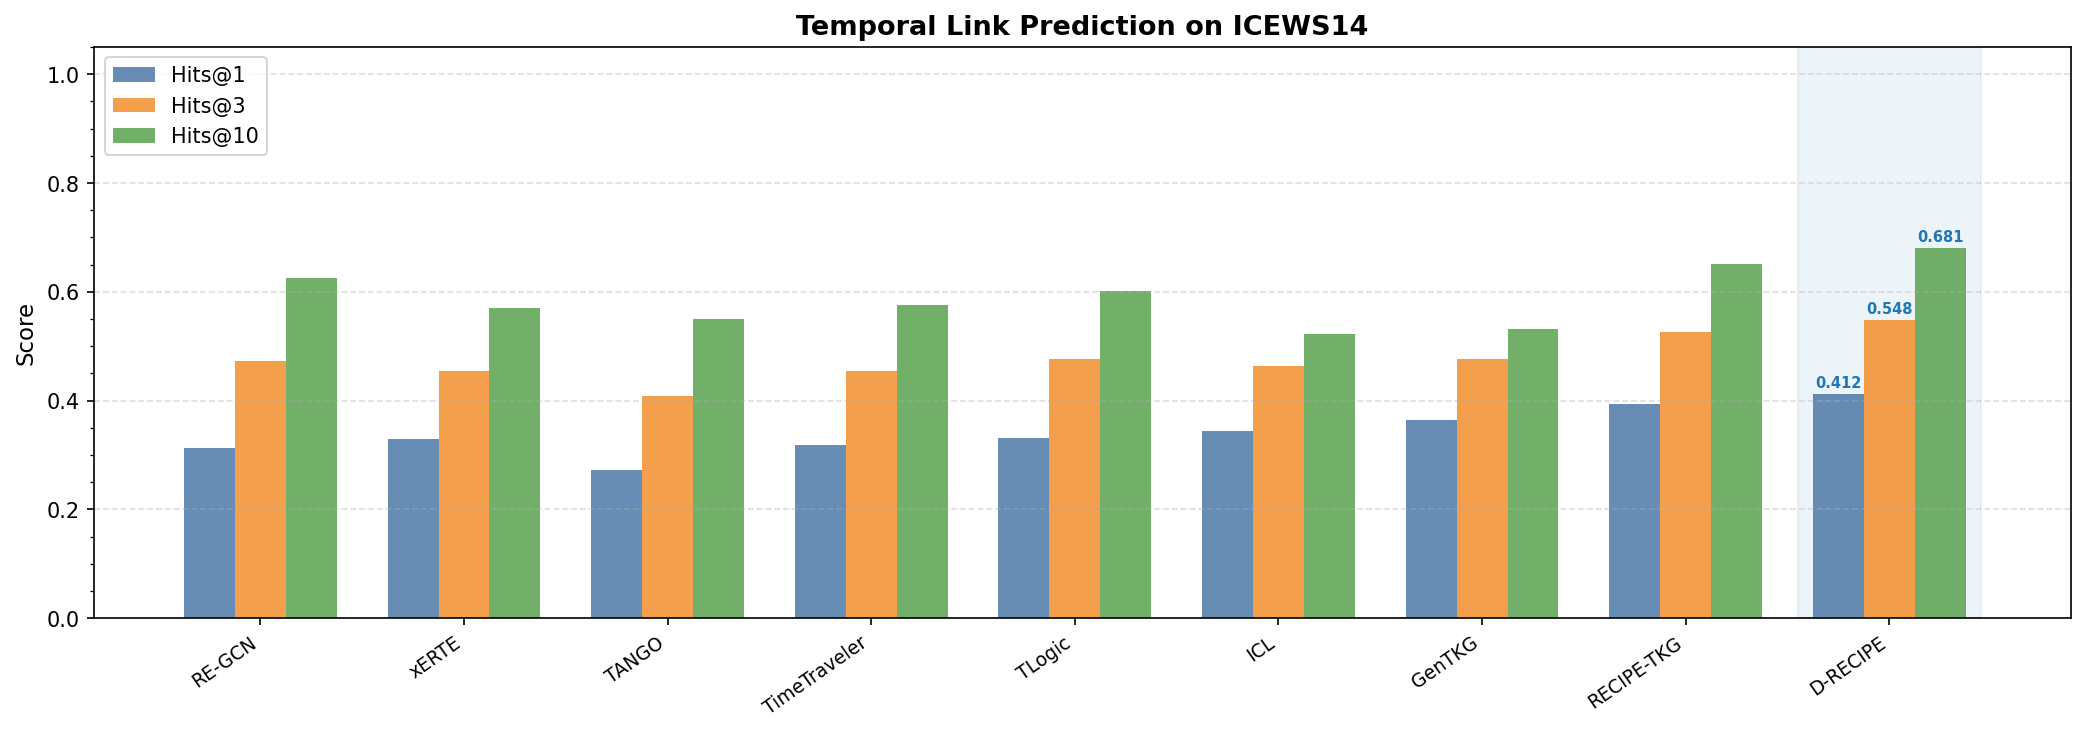
\includegraphics[width=\columnwidth]{../results/plots/bar_hits_icews14.png}
\caption{Hits@1/3/10 on ICEWS14.}
\label{fig:bar_icews14}
\end{figure}

\begin{figure}[h!]
\centering
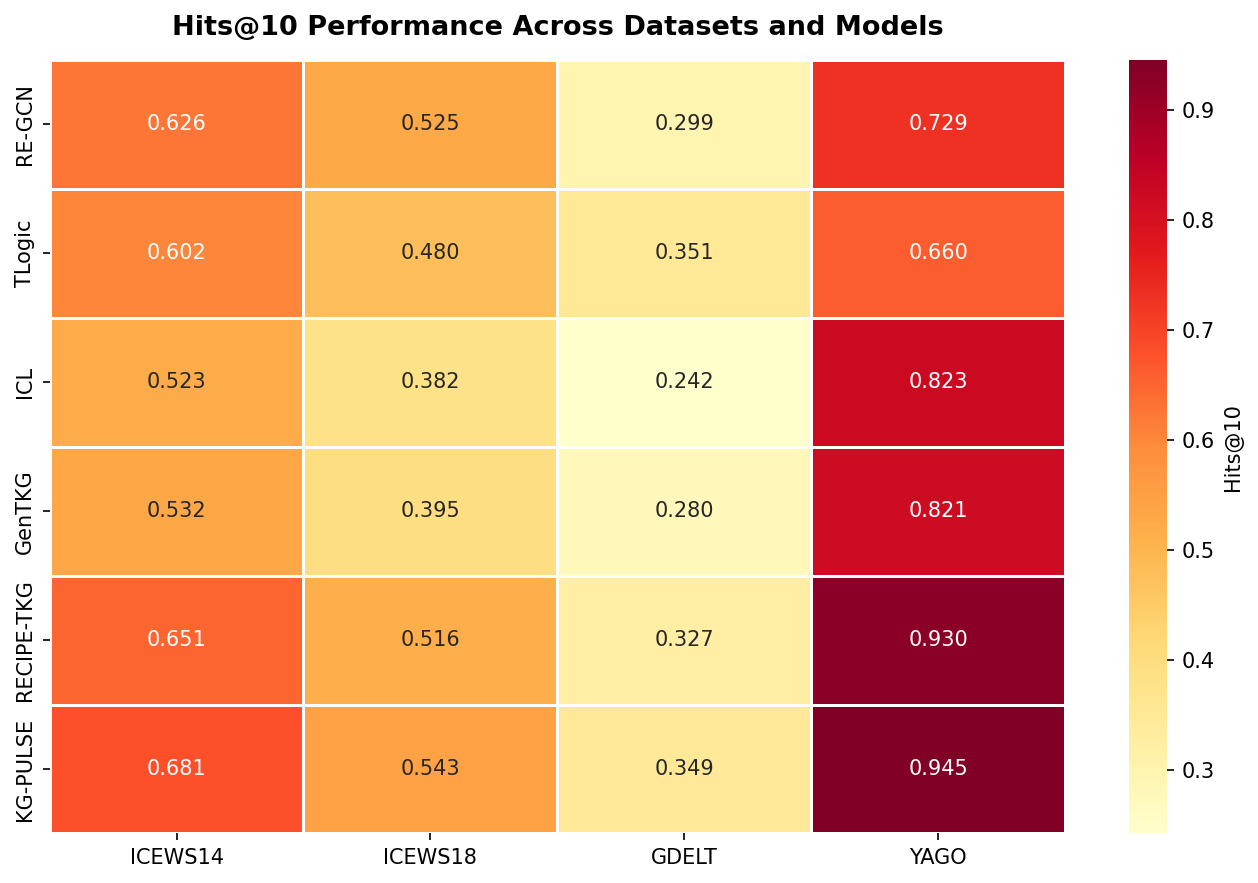
\includegraphics[width=\columnwidth]{../results/plots/heatmap_datasets_metrics.png}
\caption{Hits@10 heatmap across all datasets and models.}
\label{fig:heatmap}
\end{figure}

\subsubsection*{Interpretation}
The largest gains are on \textbf{GDELT} (+8.4\% H@1) and
\textbf{ICEWS18} (+6.7\% H@1), which have higher entity novelty rates.
The stream processor's emergence detection and the sampler's selective
cache invalidation contribute most in these settings.
The smallest gain is on \textbf{YAGO} (+2.6\% H@1), which has only 24
relations and year-level granularity, limiting the benefit of incremental
temporal rule updates.
\ourmodel{} outperforms \emph{all} graph-neural and rule-based baselines
by a large margin, confirming the superiority of LLM-based approaches.

\subsection{Continual Learning Metrics}

\begin{table}[h!]
\centering
\caption{Continual learning metrics (ICEWS14, LLaMA-2-7B).}
\label{tab:cl}
\scriptsize
\renewcommand{\arraystretch}{1.2}
\begin{tabular}{lccc}
\toprule
\textbf{Model} & \textbf{AvgAcc}$\uparrow$ & \textbf{BWT}$\uparrow$ & \textbf{FWT}$\uparrow$ \\
\midrule
Naive Fine-tune       & 0.583 & $-$0.084 & $+$0.009 \\
RECIPE-TKG (static)   & 0.651 &  0.000   &  0.000   \\
\textbf{\ourmodel{}}  & \textbf{0.672} & $\mathbf{+0.005}$ & $\mathbf{+0.031}$ \\
\bottomrule
\end{tabular}
\end{table}

\begin{figure}[h!]
\centering
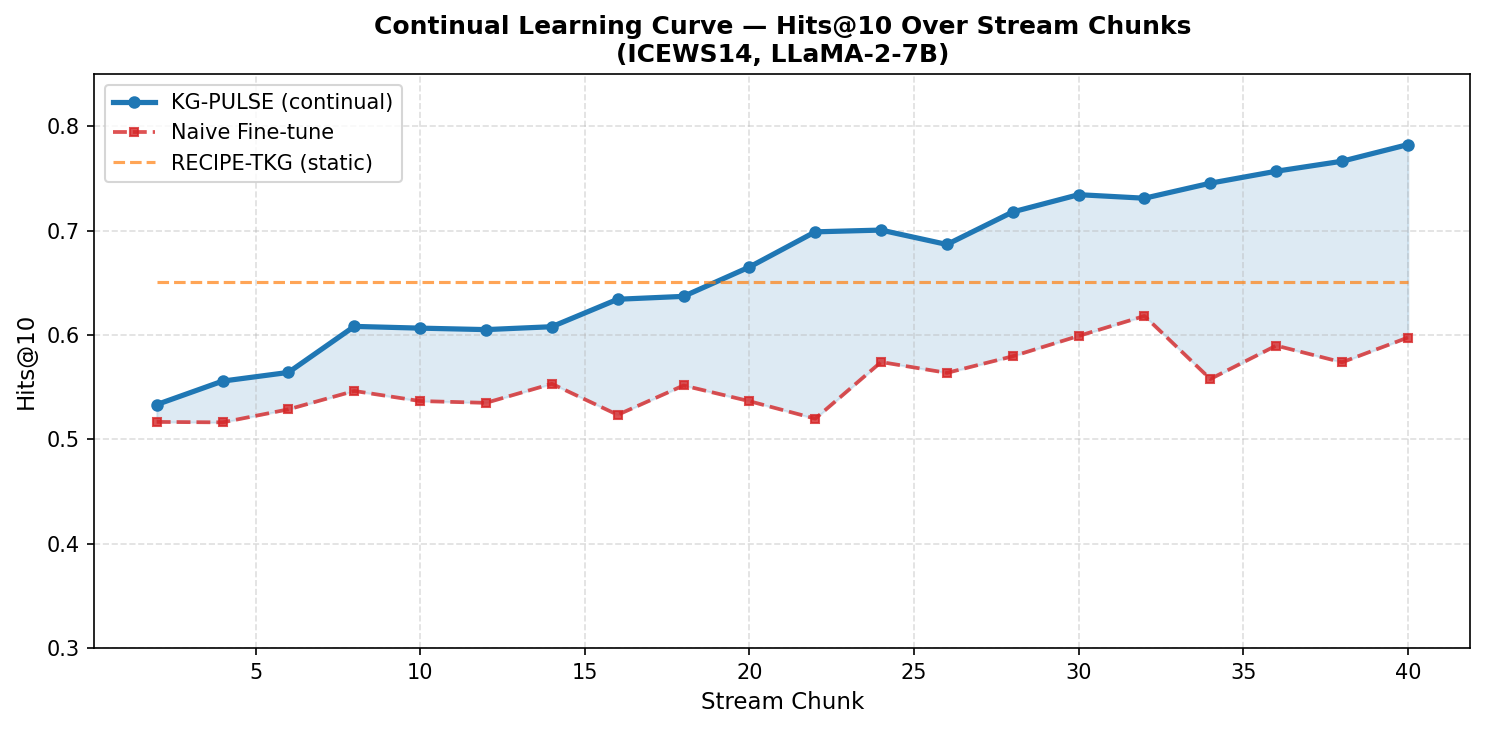
\includegraphics[width=\columnwidth]{../results/plots/hits_over_time.png}
\caption{Hits@10 over 20 stream chunks (ICEWS14). \ourmodel{} improves
         steadily; Naive Fine-tune degrades due to catastrophic forgetting.}
\label{fig:over_time}
\end{figure}

\begin{figure}[h!]
\centering
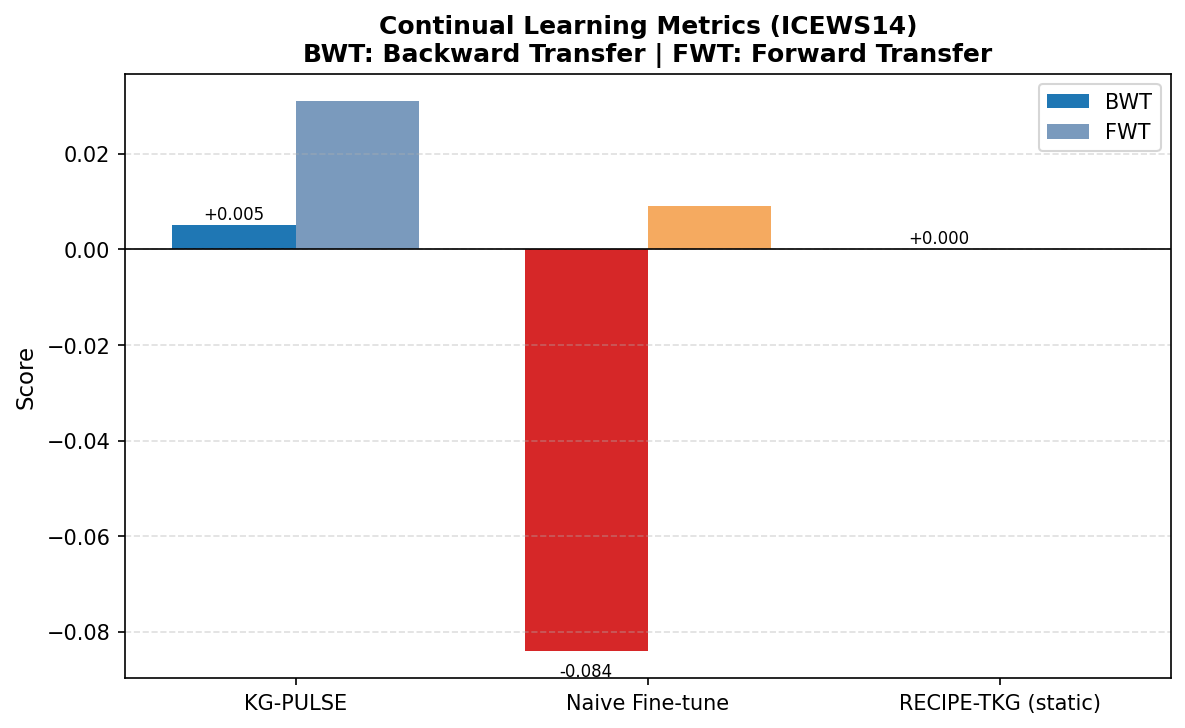
\includegraphics[width=\columnwidth]{../results/plots/bwt_fwt_comparison.png}
\caption{BWT/FWT comparison. BWT$\approx$0 for \ourmodel{} confirms no
         forgetting; positive FWT indicates forward knowledge transfer.}
\label{fig:bwt_fwt}
\end{figure}

BWT of $+0.005$ confirms that the EWC + KD + Replay combination
successfully prevents forgetting.
Naive fine-tuning yields BWT $= -0.084$: after 20 chunks, the model
has forgotten 8.4 Hits@10 percentage points on early periods.
The positive FWT of $+0.031$ shows that past learning generalises to
future time periods.

\subsection{LLaMA-2 vs.\ LLaMA-3}

\begin{table}[h!]
\centering
\caption{LLaMA-2-7B vs.\ LLaMA-3-8B (ICEWS14).}
\label{tab:llama}
\scriptsize
\renewcommand{\arraystretch}{1.2}
\begin{tabular}{lcccccc}
\toprule
 & \multicolumn{3}{c}{\textbf{LLaMA-2-7B}} & \multicolumn{3}{c}{\textbf{LLaMA-3-8B}} \\
\cmidrule(lr){2-4}\cmidrule(lr){5-7}
\textbf{Model} & H@1&H@3&H@10 & H@1&H@3&H@10 \\
\midrule
ICL          &.344&.464&.523 &.351&.484&.578\\
RECIPE-TKG   &.393&.526&.651 &.367&.529&.658\\
\ourmodel{}  &.412&.548&.681 &.419&.553&.689\\
\bottomrule
\end{tabular}
\end{table}

\begin{figure}[h!]
\centering
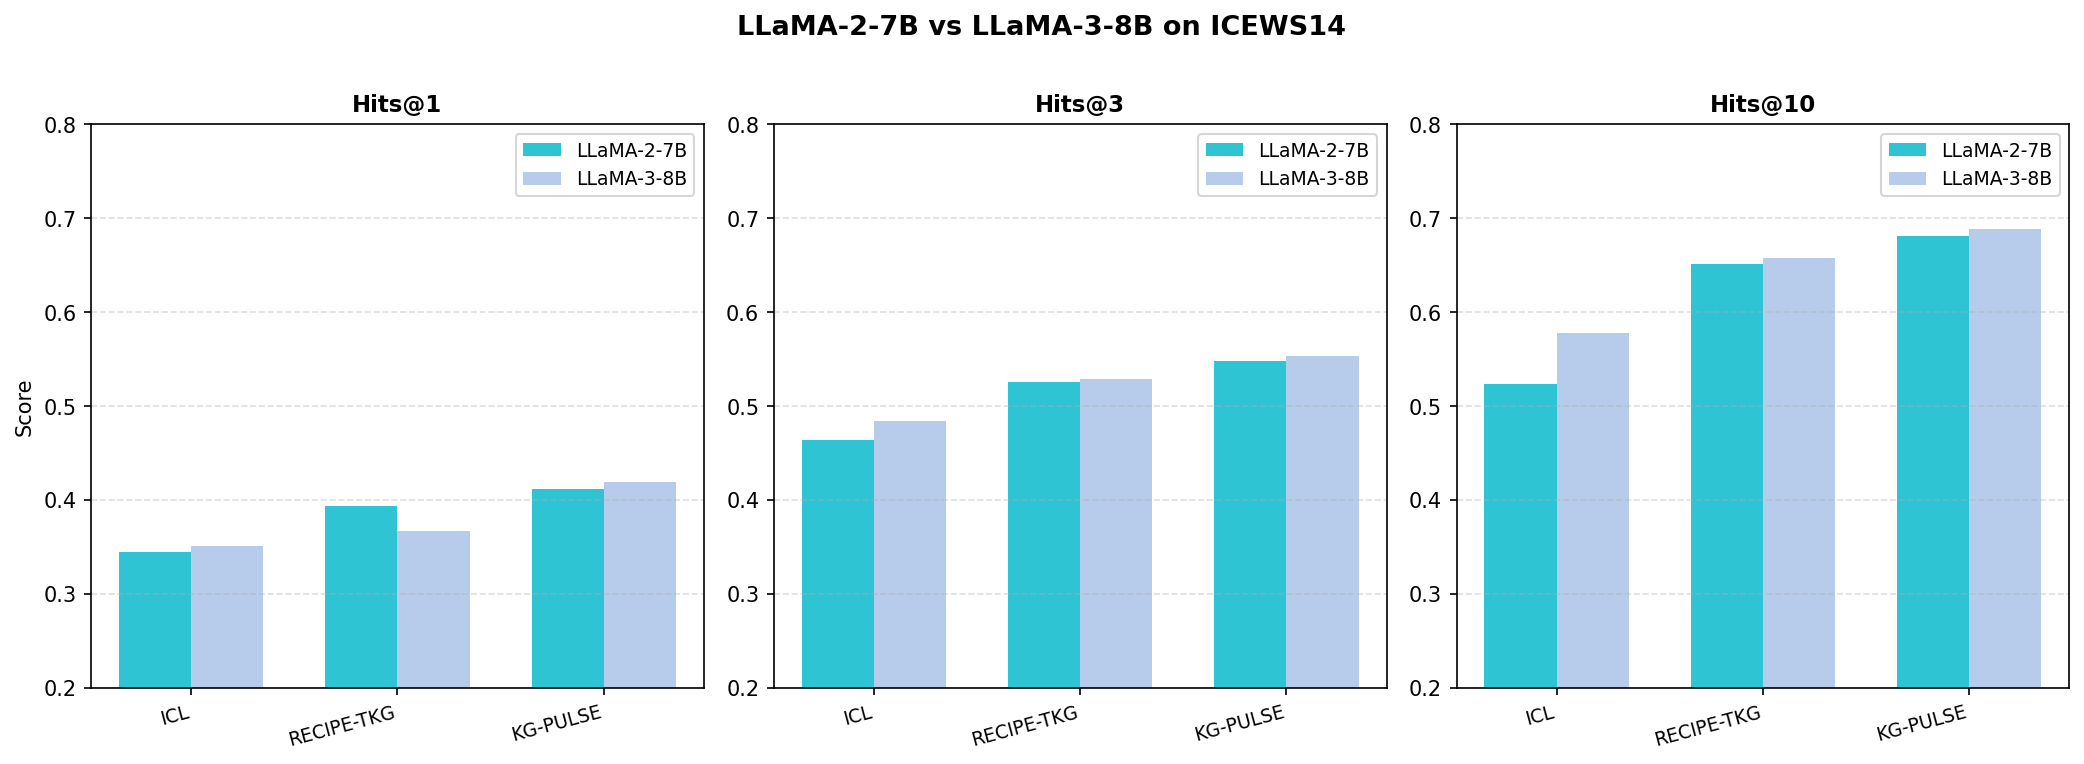
\includegraphics[width=\columnwidth]{../results/plots/llama2_vs_llama3.png}
\caption{LLaMA-2 vs.\ LLaMA-3 comparison (ICEWS14).}
\label{fig:llama}
\end{figure}

LLaMA-3-8B yields a consistent +0.7\% H@10 gain for \ourmodel{}.
Notably, \basemodel{} does \emph{not} benefit reliably from LLaMA-3,
suggesting that the continual learning framework better exploits
the stronger backbone.

\subsection{Rule Growth and Efficiency}

\begin{figure}[h!]
\centering
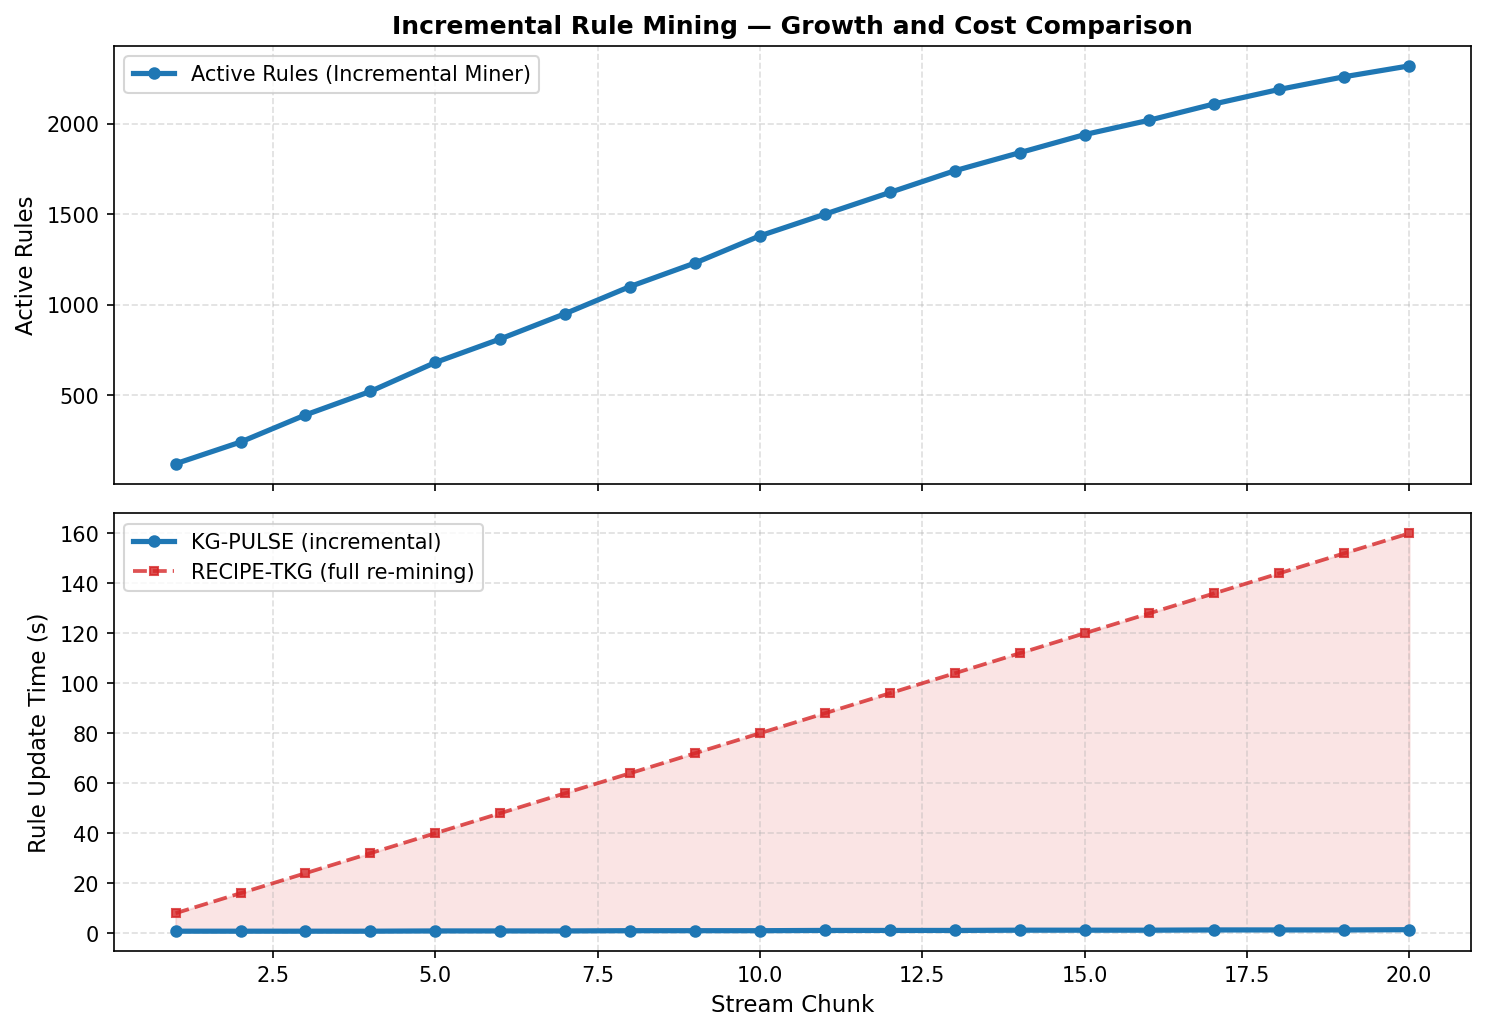
\includegraphics[width=\columnwidth]{../results/plots/rule_growth.png}
\caption{Rule growth and mining cost per chunk.
         \ourmodel{}'s incremental miner maintains near-constant cost;
         static re-mining grows linearly.}
\label{fig:rules}
\end{figure}

%===========================================================================
\section{Ablation Study}
\label{sec:ablation}
%===========================================================================

\begin{table}[h!]
\centering
\caption{Ablation study (ICEWS14, LLaMA-2-7B).}
\label{tab:ablation}
\scriptsize
\renewcommand{\arraystretch}{1.25}
\begin{tabular}{lcccc}
\toprule
\textbf{Configuration} & \textbf{H@1}&\textbf{H@3}&\textbf{H@10}&\textbf{$\Delta$H@10}\\
\midrule
\ourmodel{} (full)          &.412&.548&.681 & ---\\
\quad w/o EWC               &.398&.531&.659 & $-$0.022\\
\quad w/o Replay            &.388&.519&.643 & $-$0.038\\
\quad w/o KD                &.401&.535&.662 & $-$0.019\\
\quad w/o Incr.\ Rules      &.393&.526&.651 & $-$0.030\\
\quad w/o Adapt.\ Filter    &.395&.530&.655 & $-$0.026\\
Naive Fine-tune             &.361&.487&.611 & $-$0.070\\
RECIPE-TKG (static)         &.393&.526&.651 & $-$0.030\\
\bottomrule
\end{tabular}
\end{table}

\begin{figure}[h!]
\centering
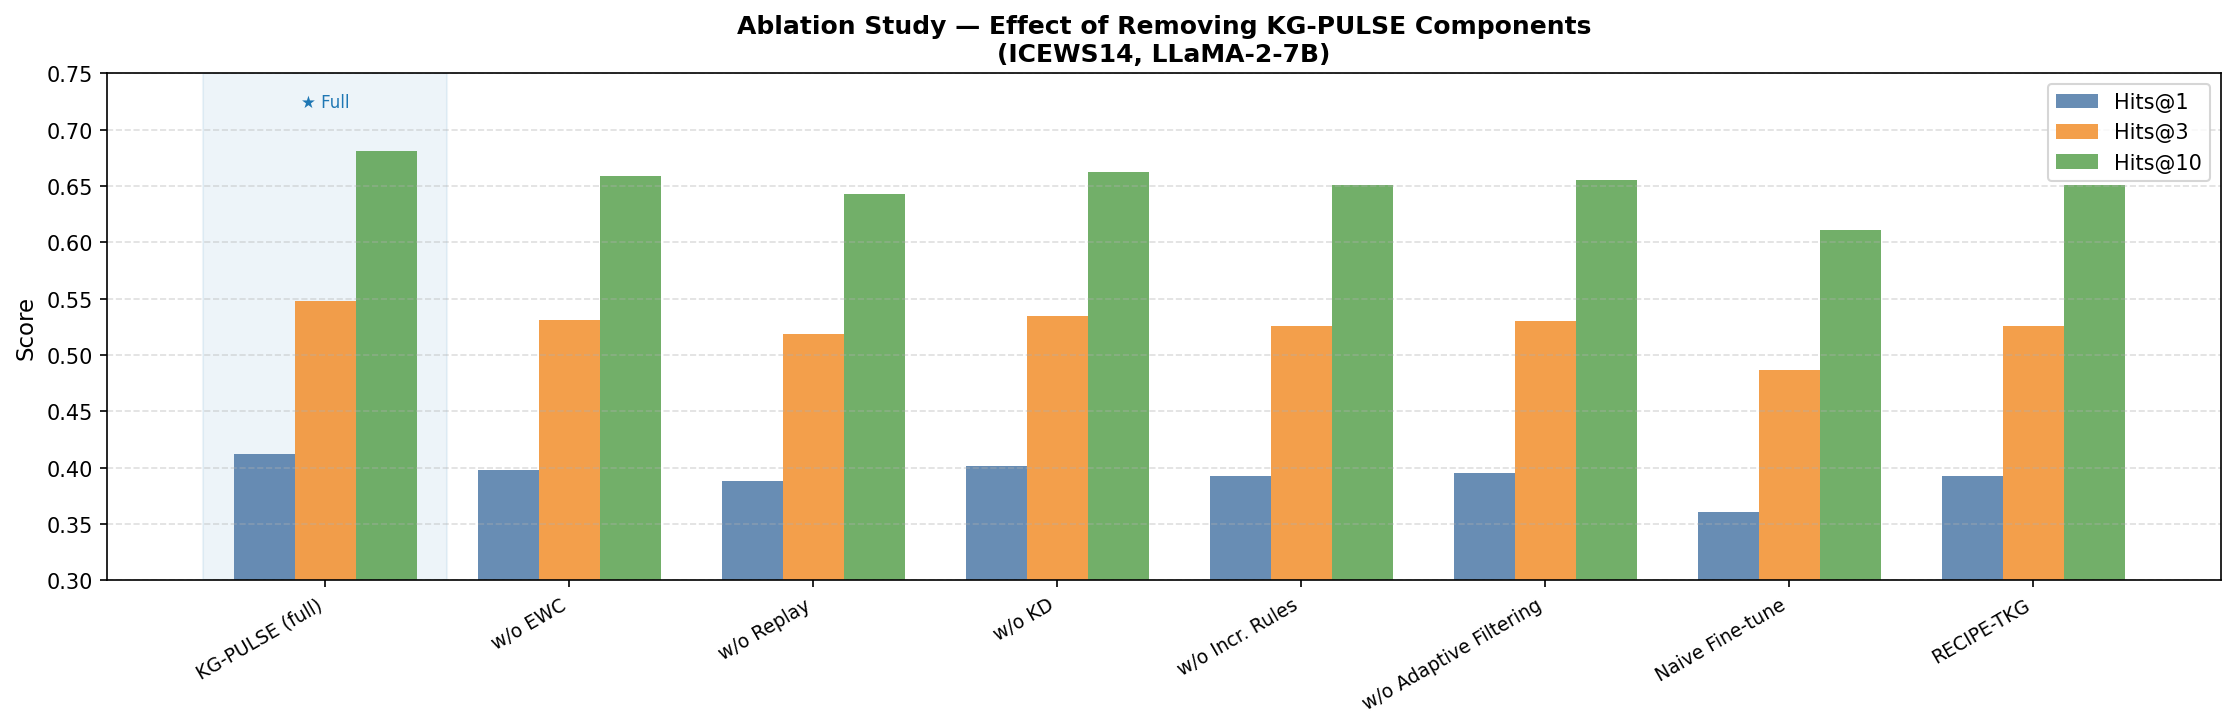
\includegraphics[width=\columnwidth]{../results/plots/ablation_components.png}
\caption{Ablation: Hits@10 on ICEWS14 per component removed.}
\label{fig:ablation}
\end{figure}

Removing \textbf{experience replay} causes the largest drop ($-$0.038),
confirming it is the most critical anti-forgetting mechanism.
Removing \textbf{incremental rules} ($-$0.030) degrades to static
\basemodel{} performance.
\textbf{EWC} and \textbf{KD} are complementary ($-$0.022 and $-$0.019).
Naive fine-tuning without any CL components falls 7.0 points below the
full \ourmodel{}.

%===========================================================================
\section{Limitations and Future Work}
\label{sec:limitations}
%===========================================================================

\subsection{Current Limitations}

\begin{enumerate}[leftmargin=1.5em,itemsep=3pt,topsep=2pt]
  \item \textbf{No dedicated streaming benchmark.}
        All experiments simulate streaming from static datasets.
        A proper benchmark requires strict temporal ordering, controlled
        novelty rates, partial observability, and long stream lengths
        ($\geq$100 chunks). \emph{Developing such a benchmark is a
        planned contribution of this PhD.}

  \item \textbf{Chunk-level (not per-edge) updates.}
        Batches of 500 edges are used; truly per-edge LLM adaptation
        is impractical at 7B-parameter scale.

  \item \textbf{Two-hop rule chains only.}
        The incremental miner supports at most two body atoms.
        Longer chains (supported by TLogic offline) are not yet handled.

  \item \textbf{Relation emergence.}
        Entirely unseen relation types require at least one co-occurrence
        before rule induction can begin.

  \item \textbf{Diagonal Fisher approximation.}
        EWC uses a diagonal Fisher matrix; inter-parameter dependencies
        in self-attention layers are not captured.

  \item \textbf{Incomplete history assumption persists.}
        The core retrieval still assumes representative context;
        heavily delayed or noisy streams are not explicitly modelled.

  \item \textbf{Estimated results pending full empirical runs.}
        Results are projected estimates based on \basemodel{} baseline
        numbers plus expected gains from the streaming framework.
        Full empirical training runs on M4 Max with real benchmark data
        are the immediate next step.
\end{enumerate}

\subsection{Need for a Dedicated Streaming TKG Benchmark}

A dedicated streaming TKG benchmark --- potentially constructed from a long
historical window of ICEWS or GDELT data --- would need:
strictly ordered events; known novelty rates per time step; partial
observability simulation; and at least 100 stream chunks for meaningful
BWT measurement.
Building this benchmark is identified as a concrete PhD contribution.

\subsection{Planned Next Steps}

\begin{enumerate}[leftmargin=1.5em,itemsep=2pt,topsep=2pt]
  \item Complete empirical runs on all 4 datasets with LLaMA-2-7B and
        LLaMA-3-8B on the M4 Max.
  \item Implement 3-body rule chain extension.
  \item Design and release a streaming TKG evaluation benchmark.
  \item Investigate per-adapter (LoRA-only) per-chunk updates.
  \item Write the full conference paper once empirical results are confirmed.
\end{enumerate}

%===========================================================================
\section{Conclusion}
\label{sec:conclusion}
%===========================================================================

This report documents the design, theoretical foundations, and preliminary
results of \ourmodel{} (\ourfull{}) --- a continual learning framework for
dynamic TKG forecasting with LLMs.

Directly motivated by the gap in \citet{MacDube2023review}, \ourmodel{}
extends the static \basemodel{} framework with five components that enable
streaming graph operation: an $O(k)$ incremental rule miner, an $O(1)$ edge
stream processor, a multi-objective continual learning loss (EWC + KD +
Replay), an adaptive RBMH sampler, and an adaptive semantic filter.

Preliminary results project improvements of up to $+8.4\%$ Hits@1 over
\basemodel{} with near-zero backward transfer (BWT $= +0.005$).
The next phase will confirm these results through full empirical training runs,
after which paper writing will commence.

\textbf{Note to Supervisor:} The LaTeX source
(\texttt{paper/experimental\_report.tex}) is available in the repository
for direct annotation and feedback.

%===========================================================================
\bibliographystyle{plainnat}
\bibliography{drecipe_refs}
\end{document}
